% ==============================================================================
% 第 11 章：组合设计 (Chapter 11: Design by Composition)
% ==============================================================================

\chapter{组合设计}
\label{sec:ch11_design_by_composition}

至此，你已经深刻体会到现实中的程序往往是复杂的智力产物，它们的实现依赖于多个相互协作的函数。只有当软件设计者深刻理解\textbf{何时需要划分多个函数}以及\textbf{如何将这些函数有机组合为一个完整程序}时，协作才能顺畅进行。

在之前的章节中，你已经多次遇到设计相关联函数的需求：有时是因为问题描述中隐含了多个不同维度的子任务，每个任务最适合由一个独立函数完成；有时则是因为一个数据定义引用了另一个数据定义，此时处理前者的函数理应调用处理后者的辅助函数。

本章将介绍若干需要组合多个函数的典型编程场景，并提供关于拆分与组合函数的指导准则。为了让代码书写更简练，我们首先介绍初学学生语言关于列表的简写扩展。

\section{list 简写函数}
\label{sec:ch11_the_list_function}

写了这么多次连续嵌套的 \code{cons} 之后，你可能已经对频繁书写 \code{(cons ... (cons ... '()))} 感到厌烦，特别是在处理长列表时。幸运的是，DrRacket 提供了包含列表简写功能的“带有列表简写的初学学生语言”（BSL+）。

\begin{notebox}[切换教学语言]
现在是升级的时候了！请在 DrRacket 的“Language（语言）”菜单中选择“Beginning Student with List Abbreviations（带有列表简写的初学学生语言）”。
\end{notebox}

最核心的革新在于引入了 \code{list} 函数。它接受任意数量的参数并构造出一个列表。理解 \code{list} 最简单的方法是将其视为宏简写：任何形如下式的表达式
\begin{lstlisting}[language=BSL]
(list exp-1 ... exp-n)
\end{lstlisting}
等价于 $n$ 次嵌套的 \code{cons} 表达式：
\begin{lstlisting}[language=BSL]
(cons exp-1 (cons ... (cons exp-n '())))
\end{lstlisting}
请注意，\code{'()} 并不是列表的元素之一，而是充当列表末尾的终止哨兵。

当然，\code{list} 的参数不仅可以是常量值，也可以是待求值的子表达式：
\begin{replbox}
> (list (+ 0 1) (+ 1 1))
(list 1 2)
> (list (/ 1 0) (+ 1 1))
/: division by zero
\end{replbox}
在构建列表之前，所有参数表达式都会被首先求值。如果其中任何一个表达式报错，列表将根本不会被构造出来。简而言之，\code{list} 的求值行为与任何接收任意参数的标准操作一致。

使用 \code{list} 极大地简化了多层嵌套列表或包含结构体的列表的书写：
\begin{lstlisting}[language=BSL]
(list 0 1 2 3 4 5 6 7 8 9)
\end{lstlisting}
只需一次 \code{list} 调用，而传统写法需要 10 次 \code{cons} 和一个 \code{'()}。

\begin{exercise}{使用 list 重写列表}{181}
使用 \code{list} 构造等价于下列各式的列表：
\begin{enumerate}
  \item \code{(cons "a" (cons "b" (cons "c" (cons "d" '()))))}
  \item \code{(cons (cons 1 (cons 2 '())) '())}
  \item \code{(cons "a" (cons (cons 1 '()) (cons \#false '())))}
  \item \code{(cons (cons "a" (cons 2 '())) (cons "hello" '()))}
\end{enumerate}
使用 \code{check-expect} 编写测试，确保你的简写版本与展开版本求值结果完全一致。
\end{exercise}

\begin{exercise}{展开 list 简写为 cons}{182}
使用基础的 \code{cons} 和 \code{'()} 还原下列列表：
\begin{enumerate}
  \item \code{(list 0 1 2 3 4 5)}
  \item \code{(list (list "he" 0) (list "it" 1) (list "lui" 14))}
  \item \code{(list 1 (list 1 2) (list 1 2 3))}
\end{enumerate}
\end{exercise}

\begin{exercise}{混合构造展开}{183}
将下列混用 \code{cons} 与 \code{list} 的表达式分别重构为：仅使用 \code{cons} 的版本，以及尽可能仅使用 \code{list} 的版本：
\begin{enumerate}
  \item \code{(cons "a" (list 0 \#false))}
  \item \code{(list (cons 1 (cons 13 '())))}
  \item \code{(cons (list 1 (list 13 '())) '())}
  \item \code{(list '() '() (cons 1 '()))}
  \item \code{(cons "a" (cons (list 1) (list \#false '())))}
\end{enumerate}
\end{exercise}

\begin{exercise}{表达式求值预测}{184}
在不运行 DrRacket 的情况下，推导下列表达式的值，并在 DrRacket 中通过 \code{check-expect} 加以验证：
\begin{enumerate}
  \item \code{(list (string=? "a" "b") \#false)}
  \item \code{(list (+ 10 20) (* 10 20) (/ 10 20))}
  \item \code{(list "dana" "jane" "mary" "laura")}
\end{enumerate}
\end{exercise}

\begin{exercise}{探索更多选择器}{185}
BSL+ 在 \code{first} 和 \code{rest} 之外还提供了许多便利的选择器。推导下式的值：
\begin{enumerate}
  \item \code{(first (list 1 2 3))}
  \item \code{(rest (list 1 2 3))}
  \item \code{(second (list 1 2 3))}
\end{enumerate}
查阅 DrRacket 文档，确认是否内置了 \code{third}、\code{fourth} 等更高阶的位置选择器。
\end{exercise}

\section{组合函数}
\label{sec:ch11_composing_functions}

回顾之前的设计指导准则：
\begin{itemize}
  \item \textbf{单一任务原则}：一个函数只负责一个明确的任务。当问题涉及不同数量间的依赖时，为其构建独立的辅助函数。
  \item \textbf{单一模板原则}：一个数据定义对应一个函数模板。当一个数据定义指向另一个数据定义时，为主函数构建处理被指向数据的辅助函数。
\end{itemize}

在将模板实例化为具体函数体（即组装子表达式的计算结果）时，以下四种情境强烈提示你需要引入\term{辅助函数}：
\begin{enumerate}
  \item \textbf{特定领域知识}：若值的组合涉及专业领域规则（如图像图形渲染、会计税收计算、音乐、几何学或物理学等），应将其抽离为辅助函数。
  \item \textbf{复杂的条件分析}：若值的组合需要对已有值进行繁琐的多情况分支判定（如正数、零、负数的不同计算），应将该 \code{cond} 逻辑封装为独立的辅助函数。
  \item \textbf{处理自引用数据元素}：若值的组合必须遍历处理另一个任意大小的数据（列表、自然数等），必须为此设计一个递归辅助函数。
  \item \textbf{泛化与抽象}：若直接求解原问题遇到阻碍，先设计一个求解\textbf{更一般化问题}的函数，再将原问题作为该通用特例予以调用！
\end{enumerate}

\begin{notebox}[愿望清单 (Wish List)]
在多函数协作开发中，核心在于维护一张\term{愿望清单}（Wish List）：记录所有为了完成当前程序而“期望存在”的辅助函数头部材料（签名、目的说明与桩定义）。
\begin{itemize}
  \item 只要愿望清单上的函数有桩定义，主程序就能直接进行局部测试；
  \item 当愿望清单清空时，整个软件的所有函数均已完工并通过测试！
\end{itemize}
在向愿望清单添加新项前，务必先检查语言标准库中是否已有现成函数。
\end{notebox}

\section{递归辅助函数}
\label{sec:ch11_auxiliary_functions_recur}

排序是计算机科学中最基础也最核心的问题之一。本节我们将通过解决一个经典的排序问题来展示递归辅助函数的设计：

\begin{notebox}[例题：实数列表降序排序]
设计函数 \code{sort>}，接收一个数字列表并输出一个按降序排列（从大到小）的新列表。
\end{notebox}

我们首先给出签名、目的说明与桩函数：
\begin{lstlisting}[language=BSL]
; List-of-numbers -> List-of-numbers
; 将 alon 重排为按降序排列的列表
(check-expect (sort> '()) '())
(check-expect (sort> (list 12 20 -5)) (list 20 12 -5))
(check-expect (sort> (list 3 2 1)) (list 3 2 1))
(check-expect (sort> (list 1 2 3)) (list 3 2 1))

(define (sort> alon)
  '())
\end{lstlisting}

根据列表模板推导：
\begin{lstlisting}[language=BSL]
(define (sort> alon)
  (cond
    [(empty? alon) '()]
    [else (... (first alon) ... (sort> (rest alon)) ...)]))
\end{lstlisting}

考察自引用分支：
\begin{itemize}
  \item \code{(first alon)} 提取首个数字（例如 \code{12}）；
  \item 自然递归 \code{(sort> (rest alon))} 已经正确地将剩余列表排好序（例如得到 \code{(list 20 -5)}）！
\end{itemize}
现在的关键任务是：\textbf{如何将首元素 \code{12} 插入到已经排好序的列表 \code{(list 20 -5)} 的正确位置上？}

在有序列表中插入一个数字需要遍历该列表以找到合适的插入位置。由于列表是任意大小的数据，根据准则 3，这必须委托给一个独立的辅助函数：
\begin{lstlisting}[language=BSL]
; Number List-of-numbers -> List-of-numbers
; 将数字 n 插入到已经按降序排列的列表 alon 中的合适位置
(define (insert n alon)
  alon)
\end{lstlisting}

有了这个愿望清单中的 \code{insert}，主函数 \code{sort>} 即可立刻落笔成型：
\begin{lstlisting}[language=BSL]
(define (sort> alon)
  (cond
    [(empty? alon) '()]
    [else (insert (first alon) (sort> (rest alon)))]))
\end{lstlisting}

接下来设计 \code{insert}：
\begin{lstlisting}[language=BSL]
(check-expect (insert 5 '()) (list 5))
(check-expect (insert 5 (list 6)) (list 6 5))
(check-expect (insert 5 (list 4)) (list 5 4))
(check-expect (insert 12 (list 20 -5)) (list 20 12 -5))
\end{lstlisting}

在 \code{insert} 中，若列表为空，则返回 \code{(list n)}；若列表非空，且 $n \ge \text{首元素}$，由于后续元素更小，故直接 \code{(cons n alon)}；否则，首元素保留在最前，将 $n$ 递归插入到剩余部分中：\code{(cons (first alon) (insert n (rest alon)))}。

图~\ref{fig:sorting_lists_of_numbers} 展示了完整的\term{插入排序}（Insertion Sort）程序。

\begin{figure}[htbp]
  \centering
  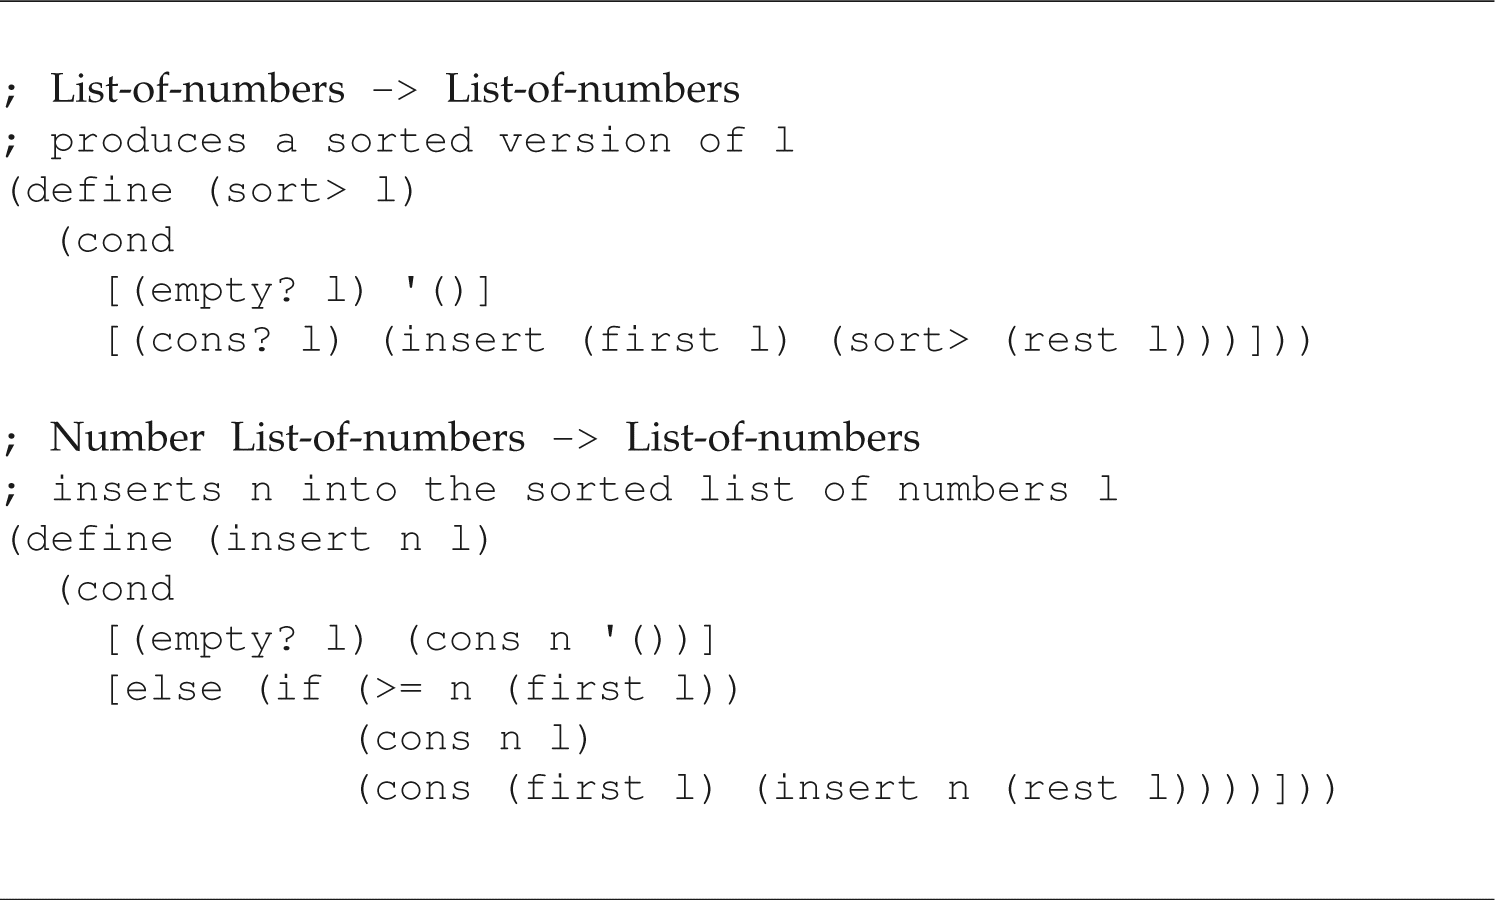
\includegraphics[width=0.85\textwidth]{images/00259.png}
  \caption{基于插入排序实现的完整排序程序}
  \label{fig:sorting_lists_of_numbers}
\end{figure}

\begin{exercise}{使用 check-satisfied 验证排序}{186}
利用练习 145 中的谓词 \code{sorted>?}，配合 \code{check-satisfied} 重新表述 \code{sort>} 的测试用例。思考如何编写测试用例来证明一个永远返回 \code{(list 9 8 7 6 5 4 3 2 1 0)} 的虚假排序函数 \code{sort>/bad} 并非真正的排序程序？
\end{exercise}

\begin{exercise}{玩家按得分排序}{187}
设计程序对游戏玩家结构体列表按分数降序排序：
\begin{lstlisting}[language=BSL]
(define-struct gp [name score])
; A GamePlayer 是结构体：(make-gp String Number)
\end{lstlisting}
\end{exercise}

\begin{exercise}{邮件排序}{188}
定义邮件结构体 \code{(make-email from date message)}。分别设计两个排序程序：一个按收信时间戳（数字）降序排序；另一个按发件人姓名（字符串）按字母表顺序排序（使用 \code{string<?}）。
\end{exercise}

\begin{exercise}{有序列表的高效搜索 search-sorted}{189}
针对已按升序排列的数字列表设计 \code{search-sorted} 函数：判断数字 $n$ 是否存在。当遇到大于 $n$ 的列表元素时，函数应当提前终止搜索。
\end{exercise}

\begin{exercise}{前缀与后缀列表生成}{190}
设计函数 \code{prefixes}：消耗字符列表并产生所有前缀构成的列表。

接着设计函数 \code{suffixes}：产生所有后缀构成的列表。
\end{exercise}

\section{通用辅助函数}
\label{sec:ch11_auxiliary_generalize}

有时一个辅助函数不仅是一个简单的帮手，更是一个\textbf{更具一般性的通用问题的解}。当我们试图直接解决某个过于狭隘的问题时，常规的设计手段可能会走入死胡同；此时退后一步，提炼出更通用的一般化任务，反而能化繁为简。

\begin{notebox}[例题：在画布中绘制多边形]
设计一个函数在给定画布上绘制任意多边形（Polygon）。
\end{notebox}

在平面几何中，多边形是由至少三个顶点（Posn）按序连线围成的闭合区域。其数据定义如下：
\begin{lstlisting}[language=BSL]
; A Polygon 是以下之一：
; -- (list Posn Posn Posn)
; -- (cons Posn Polygon)
; 解释：至少包含 3 个顶点的有序点集
\end{lstlisting}

如果我们直接尝试编写函数 \code{render-poly}：在处理基准三角形时连成闭合回路；但在递归处理多于三个点的多边形时，若直接让递归调用绘制剩余多边形，就会发现\textbf{剩余多边形的末端三点被错误地提前闭合了}（变成了图~\ref{fig:drawing_polygon} 之前描述的异常打结图形）！

\begin{figure}[htbp]
  \centering
  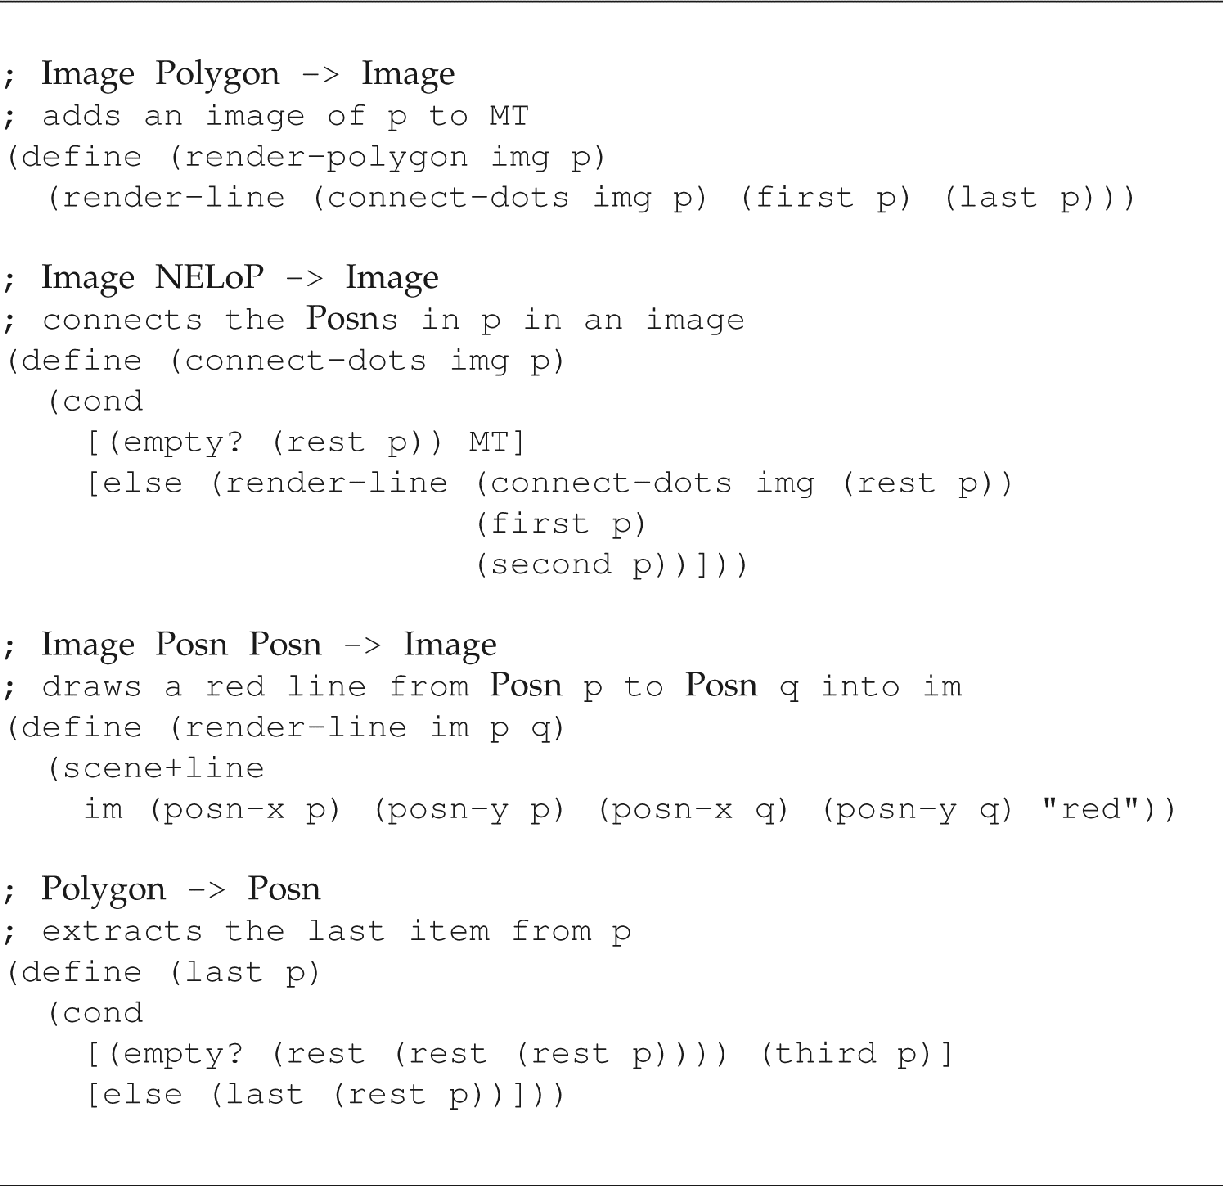
\includegraphics[width=0.85\textwidth]{images/00275.png}
  \caption{多边形绘制程序的正确设计与分解}
  \label{fig:drawing_polygon}
\end{figure}

分析该失败的根源揭示出关键洞见：绘制多边形本质上由两步组成：
\begin{enumerate}
  \item \textbf{更一般的子问题}：将任意非空点集依次连线成“开折线”（connect the dots）；
  \item \textbf{原问题的特化}：最后画一条从首顶点到末顶点的封闭边！
\end{enumerate}

为此，我们针对更通用的非空点集 \code{NELoP}（Non-Empty List of Posns）设计连线函数 \code{connect-dots}：
\begin{lstlisting}[language=BSL]
; Image NELoP -> Image
; 将 p 中的所有连续点依次用线段相连
(define (connect-dots img p)
  (cond
    [(empty? (rest p)) img]
    [else
     (render-line (connect-dots img (rest p))
                  (first p)
                  (second p))]))
\end{lstlisting}

同时为提取末顶点的需求设计辅助函数 \code{last}：
\begin{lstlisting}[language=BSL]
; NELoP -> Posn
; 提取列表中的最后一个点
(define (last p)
  (cond
    [(empty? (rest p)) (first p)]
    [else (last (rest p))]))
\end{lstlisting}

有了这两个高内聚、通用性强的辅助函数，原本复杂棘手的 \code{render-poly} 主函数竟然变成了一行优雅的组合：
\begin{lstlisting}[language=BSL]
; Image Polygon -> Image
; 在场景中绘制闭合多边形 p
(define (render-poly img p)
  (render-line (connect-dots img p)
               (first p)
               (last p)))
\end{lstlisting}

\begin{exercise}{connect-dots 示例与测试}{191}
为 \code{connect-dots} 补充完整的测试用例，涵盖单点、两点、四点的各种几何图形。
\end{exercise}

\begin{exercise}{last 函数推导与验证}{192}
解释为什么可以直接对 \code{Polygon} 调用针对 \code{NELoP} 设计的 \code{last} 函数。
\end{exercise}

\begin{exercise}{render-poly 的替代设计思路}{193}
尝试通过以下两种不同思路重构 \code{render-poly}，并确保通过测试：
\begin{enumerate}
  \item 先将末顶点 \code{(last p)} \code{cons} 到 \code{p} 的前端，然后直接调用 \code{connect-dots}；
  \item 先将首顶点 \code{(first p)} 添加到 \code{p} 的尾部，然后直接调用 \code{connect-dots}。
\end{enumerate}
\end{exercise}

\begin{exercise}{带闭合终点的 connect-dots}{194}
修改 \code{connect-dots}，令其额外接收一个指定的闭合目标点 \code{target}，使得最后一个点自动与该目标点相连。随后据此简化 \code{render-poly}。
\end{exercise}
